\documentclass[12pt,table,t]{beamer}

% Packages
\usepackage{xcolor}
\usepackage{eulervm}
\usepackage[utf8]{inputenc}


% Theme
\mode<presentation>
{
  \usetheme{Honefoss}
%  \setbeamercovered{transparent}
  \setbeamertemplate{blocks}[rounded]
  \AtBeginPart{\frame[c]{\partpage}}
}

\logooff
\newcommand{\comment}[1]{{\slshape\color{kvred}#1}}

\title{Listening to Quasars and Shooting Satellites with Lasers}
\author{Geir Arne Hjelle}
\date{EuroSciPy, August 31st 2018}
\titlegraphic{\includegraphics[width=\paperwidth]{figure/vlbi}}

\begin{document}
\frame[plain]{\titlepage}

\part{Why?}

\begin{frame}[c]{The Problem}
  \begin{center}
    \includegraphics<1>[width=\textwidth]{figure/altimetry_01}
    \includegraphics<2>[width=\textwidth]{figure/altimetry_02}
    \includegraphics<3>[width=\textwidth]{figure/altimetry_03}
    \includegraphics<4>[width=\textwidth]{figure/altimetry_04}
    \includegraphics<5>[width=\textwidth]{figure/altimetry_05}
    \includegraphics<6>[width=\textwidth]{figure/gps_01}
    \includegraphics<7>[width=\textwidth]{figure/gps_02}
    \includegraphics<8>[width=\textwidth]{figure/gps_03}
  \end{center}
\end{frame}


\begin{frame}[c]{The Solution}
  \begin{center}
    \includegraphics<1>[width=\textwidth]{figure/reference_system}
  \end{center}

  A \textbf{Reference System}\footnote{Really just a coordinate system based on reference points}
\end{frame}


\begin{frame}[c]{The Solution}
  \begin{center}
    \includegraphics[width=\textwidth]{figure/gps_04}
  \end{center}
\end{frame}


\begin{frame}[c]{The Solution}
  But it's not trivial to define such a Reference System ...

  \vspace*{4ex}
  \begin{center}
    \includegraphics<1>[width=\textwidth]{figure/origin}
  \end{center}
\end{frame}


\begin{frame}[c]{The Solution}
  Want a \textbf{Reference System} that is:

  \begin{itemize}
  \item<2-> precise
  \item<3-> stable over time
  \end{itemize}

  \begin{center}
    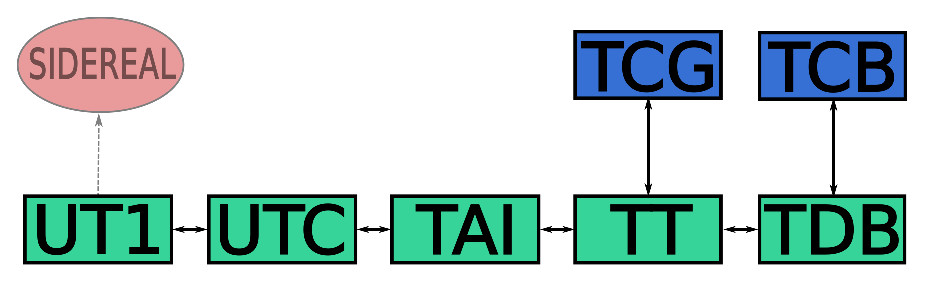
\includegraphics[width=\textwidth]{figure/time}
  \end{center}
\end{frame}


\begin{frame}[c]{Challenges}

  \begin{itemize}
  \item<2-> Tectonic plates drifting
  \item<3-> Land rise and sea level rise
  \item<4-> Earthquakes
  \end{itemize}
  
  \begin{center}
    \includegraphics<-1>[width=.3\textwidth]{figure/earth_sq}
    \includegraphics<2->[width=.3\textwidth]{figure/plate_drift_sq}
    \includegraphics<-2>[width=.3\textwidth]{figure/earth_sq}
    \includegraphics<3->[width=.3\textwidth]{figure/uplift}
    \includegraphics<-3>[width=.3\textwidth]{figure/earth_sq}
    \includegraphics<4->[width=.3\textwidth]{figure/earthquake_sq}
  \end{center}
\end{frame}


\begin{frame}{Solutions}

  \begin{itemize}
  \item Local Systems
  \end{itemize}
  
  \begin{center}
    \includegraphics<1>[width=\textwidth]{figure/local_system_01}
    \includegraphics<2>[width=\textwidth]{figure/local_system_02}
  \end{center}
\end{frame}


\begin{frame}{Solutions}

  \begin{itemize}
  \item Coordinates that move
  \end{itemize}
  
  \begin{center}
    \includegraphics<1>[width=\textwidth]{figure/snail_01}
    \includegraphics<2>[width=\textwidth]{figure/snail_02}
    \includegraphics<3>[width=\textwidth]{figure/snail_03}
    \includegraphics<4>[width=\textwidth]{figure/snail_04}
    \includegraphics<5>[width=\textwidth]{figure/snail_05}
  \end{center}
\end{frame}

\part{What?}

\begin{frame}[c]{ITRF}

  \begin{itemize}
  \item The International Terrestrial Reference Frame
  \end{itemize}
    
  \begin{center}
    \includegraphics<1>[width=\textwidth]{figure/itrf_01}
    \includegraphics<2>[width=\textwidth]{figure/itrf_02}
    \includegraphics<3>[width=\textwidth]{figure/itrf_03}
  \end{center}
\end{frame}

\part{How?}

\begin{frame}[c]{International Cooperation}
  \begin{center}
    \includegraphics<1>[width=\textwidth]{figure/cooperation_01}
    \includegraphics<2>[width=\textwidth]{figure/cooperation_02}
    \includegraphics<3>[width=\textwidth]{figure/cooperation_03}
    \includegraphics<4>[width=\textwidth]{figure/cooperation_04}
    \includegraphics<5>[width=\textwidth]{figure/cooperation_05}
  \end{center}

  \begin{itemize}
  \item The ITRF is created based on observations from four different space geodetic techniques
    \begin{itemize}
    \item<2-> VLBI -- Very Long Baseline Interferometry
    \item<3-> SLR -- Satellite Laser Ranging
    \item<4-> GNSS -- Global Navigation Satellite Systems (e.g. GPS)
    \item<5-> DORIS -- Doppler Orbitography and Radiopositioning
    \end{itemize}
  \end{itemize}
\end{frame}


\begin{frame}[c]{Still Some Challenges}

  \begin{itemize}
  \item The Earth rotates
  \end{itemize}
  
  \begin{center}
    \includegraphics<1>[width=0.3\textwidth]{figure/earth_rotates_01}
    \includegraphics<2>[width=0.3\textwidth]{figure/earth_rotates_02}
    \includegraphics<3>[width=0.3\textwidth]{figure/earth_rotates_03}
    \includegraphics<4>[width=0.3\textwidth]{figure/earth_rotates_04}
    \includegraphics<5>[width=0.3\textwidth]{figure/earth_rotates_05}
    \includegraphics<6>[width=0.3\textwidth]{figure/earth_rotates_06}
    \includegraphics<7>[width=0.3\textwidth]{figure/earth_rotates_07}
    \includegraphics<8>[width=0.3\textwidth]{figure/earth_rotates_08}
    \includegraphics<9>[width=0.3\textwidth]{figure/earth_rotates_01}
  \end{center}

  \begin{itemize}
  \item<9-> Fix the Reference System to the Earth with $z$ as the rotation axis
  \end{itemize}
\end{frame}


\begin{frame}[c]{Still Some Challenges}

  \begin{itemize}
  \item The Earth wobbles
  \end{itemize}
  
  \begin{center}
    \includegraphics<1>[width=0.4\textwidth]{figure/cheers_01}
    \includegraphics<2>[width=0.3\textwidth]{figure/drunk_01}
    \includegraphics<3>[width=0.3\textwidth]{figure/drunk_02}
    \includegraphics<4>[width=0.3\textwidth]{figure/drunk_01}
    \includegraphics<5>[width=0.3\textwidth]{figure/drunk_02}
  \end{center}

  \begin{itemize}
  \item<5-> Continuously update the Earth Orientation Parameters
  \end{itemize}
\end{frame}


\begin{frame}[c]{VLBI}
  \begin{center}
    \includegraphics<1>[width=\textwidth]{figure/vlbi_concept_01}
    \includegraphics<2>[width=\textwidth]{figure/vlbi_concept_02}
    \includegraphics<3->[width=\textwidth]{figure/vlbi_concept_03}
  \end{center}

  \uncover<4->{
  Calculate \textbf{model} where:
  \begin{itemize}
  \item position of stations is assumed known (ITRF)
  \item a priori estimate of wobble is included
  \end{itemize}}
\end{frame}


\begin{frame}[c]{VLBI}
  The residual

  \begin{center}
    \textbf{obs} - \textbf{model}
  \end{center}

  can be used to estimate the true wobble.

  \uncover<2>{
    \begin{center}
      \includegraphics[width=.4\textwidth]{figure/cheers_02}
    \end{center}
  }
\end{frame}


\begin{frame}[c]{SLR}
  \begin{center}
    \includegraphics<1>[width=\textwidth]{figure/slr_concept_01}
    \includegraphics<2>[width=\textwidth]{figure/slr_concept_02}
    \includegraphics<3>[width=\textwidth]{figure/slr_concept_03}
  \end{center}
\end{frame}


\begin{frame}[c]{SLR}
  Two applications:

  \begin{center}
    \includegraphics<1>[width=\textwidth]{figure/lageos_01}
    \includegraphics<2>[width=\textwidth]{figure/lageos_02}
  \end{center}

  \uncover<2>{
    \begin{itemize}
    \item Stable satellite orbit\\
      $\Rightarrow$ Can calculate the position of the station (ITRF)
  \end{itemize}}
\end{frame}


\begin{frame}[c]{SLR}
  Two applications:

    \begin{center}
    \includegraphics<1>[width=0.7\textwidth]{figure/altimetry_06}
  \end{center}

  \begin{itemize}
  \item Known station position\\
    $\Rightarrow$ Can calculate satellite orbits (remote sensing)
  \end{itemize}
\end{frame}


\part{Python}


\begin{frame}[c]{Where?}
  \begin{center}
    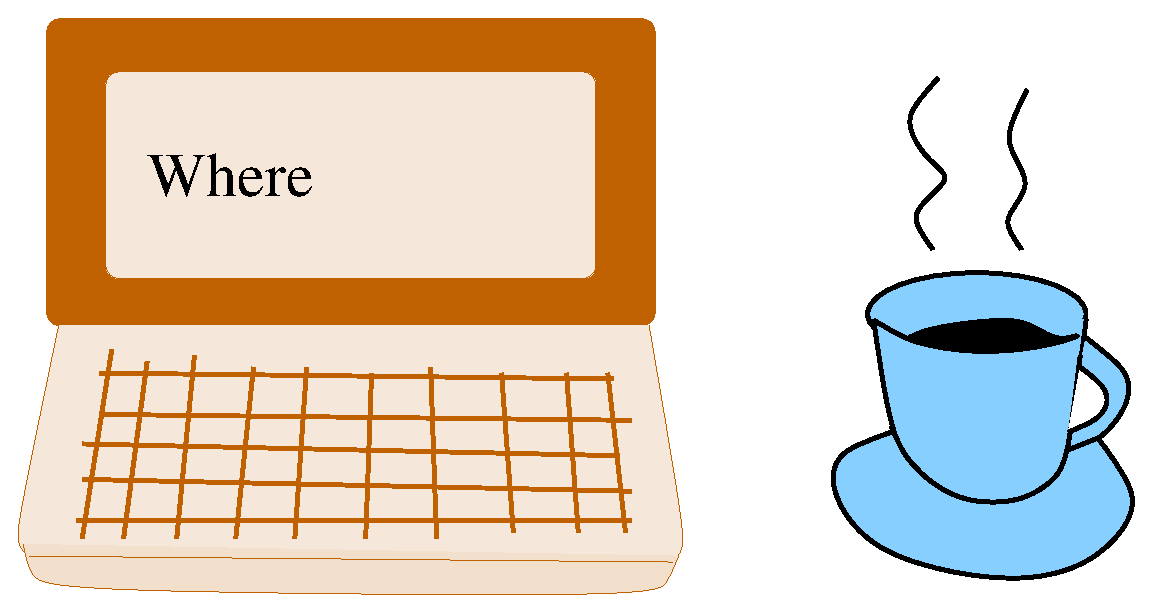
\includegraphics[width=\textwidth]{figure/where}
  \end{center}
\end{frame}


\begin{frame}[c]{Where?}
  \textbf{Where} is software that can analyse VLBI, SLR, and GNSS data, and contribute to the ITRF

  \begin{itemize}
  \item<2-> Python (mostly NumPy with a bit of Cython and F2Py)
  \item<3-> Open Source (\url{https://kartverket.github.io/where/})
  \item<4-> Fairly niche user base though
  \end{itemize}
\end{frame}


\begin{frame}[c]{There!}
  \begin{center}
    \includegraphics[width=0.4\textwidth]{figure/there_01} \hfil
    \includegraphics[width=0.4\textwidth]{figure/there_02}
  \end{center}

  Experiences:
  \begin{itemize}
  \item<2-> Thank you to everybody that contribute to the Python data science stack!!
  \item<3-> Performance: Decent Python is faster than non-optimal Fortran code :)
  \item<4-> Cython can help a lot in the right circumstances
  \end{itemize}
\end{frame}


\begin{frame}[c]{Midgard}
  %% \begin{center}
  %%   \includegraphics<1>[width=\textwidth]{figure/midgard}
  %% \end{center}

  Reusable components of Where are being separated out into its own library: \textbf{Midgard}

  \begin{itemize}
  \item `pip install midgard`
  \item Containers for coordinates that move over time
  \item Readers and parsers for geodetic file formats
  \end{itemize}
\end{frame}


\begin{frame}[c]{Thank you}
  \begin{center}
    \includegraphics[width=\textwidth]{figure/ny_alesund}

    \vfill
    {\large\url{kartverket.github.io/where/}}
    \vfill

    \includegraphics[height=1cm]{figure/logo_astropy} \hfil
    \includegraphics[height=1cm]{figure/logo_numpy} \hfil
    \includegraphics[height=1cm]{figure/logo_scipy} \hfil
    \includegraphics[height=1cm]{figure/logo_pandas} \hfil
    \includegraphics[height=1cm]{figure/logo_cython} \hfil
    \includegraphics[height=1cm]{figure/logo_f2py}
  \end{center}
\end{frame}

\end{document}
